\documentclass[11pt,a4paper]{article}
\usepackage[utf8]{inputenc}
\usepackage[spanish]{babel}
\usepackage{graphicx}
\usepackage{geometry}
\usepackage{hyperref}
\usepackage{float}
\usepackage[section]{placeins}  % Evita que floats se muevan a otras secciones
\usepackage{flafter}  % Fuerza que floats aparezcan después de ser referenciados
\usepackage{amsmath}
\usepackage{booktabs}
\usepackage{caption}
\usepackage{subcaption}
\usepackage{setspace}  % Para controlar interlineado

% Renombrar Cuadro (default en español) a Tabla
\addto\captionsspanish{%
  \renewcommand{\tablename}{Tabla}%
}

% Configuración de espaciado
\setstretch{1.15}  % Interlineado 1.15 (un poco más que simple)
\setlength{\parskip}{0.4em}  % Espacio entre párrafos
\setlength{\parindent}{1.5em}  % Sangría en primera línea

\geometry{margin=2.5cm}

% Mejores prácticas para control de flotantes
\setlength{\textfloatsep}{10pt plus 2pt minus 2pt}
\setlength{\floatsep}{10pt plus 2pt minus 2pt}
\setlength{\intextsep}{10pt plus 2pt minus 2pt}
\renewcommand{\topfraction}{0.9}
\renewcommand{\bottomfraction}{0.8}
\renewcommand{\textfraction}{0.1}
\renewcommand{\floatpagefraction}{0.7}

\hypersetup{
    colorlinks=true,
    linkcolor=blue,
    urlcolor=blue,
    citecolor=blue
}

\title{\textbf{Trabajo Práctico N° 2 \\ Histogramas, Kernels \& Métodos No Supervisados}}
\author{
    Juan Ignacio Pintos, Luis Mella, Paula Leylén Ramírez \\
    Taller de Programación, Universidad de Buenos Aires    
}
\date{Octubre 2025}

\begin{document}

\maketitle

\noindent\textbf{Repositorio GitHub:} \url{https://github.com/paulaleylen/BigDataUBA-GrupoJLP}

\section{Introducción}

Este trabajo continúa el análisis de la EPH del INDEC iniciado en el TP1, profundizando en técnicas de visualización y métodos no supervisados. Utilizando datos del Gran Buenos Aires de los primeros trimestres de 2005 y 2025, el objetivo es identificar patrones en la estructura socioeconómica sin utilizar etiquetas de pobreza hasta la etapa final.

El enfoque busca responder: ¿la pobreza emerge naturalmente de la covarianza de variables socioeconómicas (edad, educación, ingresos, composición del hogar), o constituye un constructo normativo que trasciende estas dimensiones? La Parte I aplica histogramas y kernels para explorar distribuciones de variables clave, identificando diferencias entre pobres y no pobres. La Parte II implementa PCA y clustering para descubrir estructuras latentes, evaluando si estos algoritmos replican la clasificación de pobreza del INDEC\@.

\section{Parte I: Creación de variables y análisis exploratorio}

\subsection{Variables creadas y metodología}

Se crearon cuatro variables derivadas. La primera, edad2, es una transformación cuadrática de EDAD que captura efectos no lineales del ciclo de vida sobre ingresos, siguiendo ecuaciones de Mincer estándar donde la relación edad-ingreso presenta trayectoria cóncava.

La segunda, educ, convierte las categorías de NIVEL\_ED en años de escolaridad según el sistema argentino (sin instrucción: 0, primaria: 7, secundaria: 12, universitario: 17). Se implementó un mapeo dual para las diferencias de formato entre años: 2005 usa valores textuales (``Primaria Completa'') mientras 2025 usa códigos numéricos (1, 2, 3, etc.). La muestra presenta media de 9,11 años y mediana de 9, revelando que más de la mitad del GBA no completó la secundaria. La tercera variable, ingreso\_total\_familiar, actualiza el ITF de 2005 a pesos constantes de 2025 usando el IPC oficial del INDEC empalmado por BCRA (factor 356,22x, inflación acumulada 38.530,63\%). Finalmente, horastrab cuantifica la intensidad laboral semanal del jefe de hogar, con cobertura del 56,5\% y estadísticas que revelan un mercado fragmentado (promedio 31,0 hrs, mediana 40 hrs, máximo 168 hrs).

\subsection{Distribución de edades y análisis kernel}

La Figura~\ref{fig:edades} revela diferenciación etaria clara entre pobres y no pobres. El Panel A muestra la estructura característica de regiones urbanas con concentración en edades productivas (20--50 años), mientras el Panel B evidencia que la población pobre se concentra en edades más jóvenes (20--40 años, hogares en formación) y la no pobre presenta mayor dispersión hacia edades mayores, asociada a acumulación de capital y experiencia laboral. Este patrón sugiere que la pobreza está fuertemente vinculada al ciclo de vida, donde las familias jóvenes enfrentan mayor vulnerabilidad durante la fase de formación y crianza.

\subsection{Distribución de ingresos y polarización económica}

La Figura~\ref{fig:ingresos} evidencia polarización extrema en la estructura de ingresos del GBA\@. El histograma del Panel A presenta la asimetría positiva típica de distribuciones de ingreso, con alta concentración en rangos bajos y cola extendida. El Panel B compara las distribuciones kernel de pobres y no pobres, mostrando separación clara sin superposición: los pobres exhiben un pico pronunciado en valores bajos mientras los no pobres se dispersan en niveles sustancialmente superiores. Esta segmentación valida que la línea de pobreza CBT captura una discontinuidad real en la estructura económica.

\subsection{Tabla 1: Resumen de la base final}

La Tabla~\ref{tab:resumen} presenta las estadísticas descriptivas de la base final. El dataset contiene 16.778 observaciones totales (9.542 en 2005, 7.236 en 2025), evidenciando una reducción muestral del 24,2\%. La variable Pobre tiene cobertura completa, validando la integridad del cálculo basado en la metodología INDEC\@. El deterioro socioeconómico es significativo: la tasa de pobreza pasó de 26,91\% en 2005 a 40,77\% en 2025, incremento de 13,86 puntos porcentuales. En términos absolutos, el número de pobres creció 14,9\% (de 2.568 a 2.950) mientras la cantidad de no pobres cayó 38,5\% (de 6.974 a 4.286), reflejando no solo empobrecimiento de sectores vulnerables sino también descenso significativo de capas medias hacia la pobreza.

\begin{table}[H]
    \centering
    \begin{tabular}{lccc}
        \toprule
        \textbf{Descripción}   & \textbf{2005} & \textbf{2025} & \textbf{Total} \\
        \midrule
        Cantidad observaciones & 9.542         & 7.236         & 16.778         \\
        NAs en variable Pobre  & 0             & 0             & 0              \\
        Cantidad de Pobres     & 2.568         & 2.950         & 5.518          \\
        Cantidad de No Pobres  & 6.974         & 4.286         & 11.260         \\
        Variables limpias      & 94            & 94            & 94             \\
        \midrule
        Tasa de pobreza (\%)   & 26,91\%       & 40,77\%       & 32,89\%        \\
        \bottomrule
    \end{tabular}
    \caption{Resumen de la base final para la región Gran Buenos Aires}
    \label{tab:resumen}
\end{table}

\section{Parte II: Métodos no supervisados}

\subsection{Matriz de correlaciones y estructura de covarianza}

La Figura~\ref{fig:correlaciones} presenta la matriz de correlaciones entre las seis variables seleccionadas: EDAD, edad2, educ, ingreso\_total\_familiar, miembros\_hogar y horastrab. El heatmap con escala divergente centrada en cero facilita la identificación visual de las relaciones lineales bivariadas.

Las correlaciones estructurales más relevantes incluyen: EDAD vs edad2 ($r = 0,947$), correlación altísima esperada por construcción matemática; EDAD vs educ ($r = 0,444$), moderada reflejando efectos de cohorte educativo; educ vs ingreso\_total\_familiar ($r = 0,228$), sugiriendo retornos educativos moderados donde más educación se asocia con mayores ingresos, aunque la magnitud indica que la educación explica solo una fracción limitada de la variabilidad; educ vs miembros\_hogar ($r = -0,189$), negativa consistente con transición demográfica; y horastrab vs ingreso\_total\_familiar ($r = 0,167$), débil reflejando la coexistencia de subempleo y pluriempleo en el mercado laboral del GBA\@. Las correlaciones moderadas (ninguna $>$ 0,95 excepto EDAD-edad2) validan que las variables capturan dimensiones diferentes, justificando su uso conjunto en PCA y clustering sin problemas de multicolinealidad.

\subsection{Análisis de Componentes Principales (PCA)}

El PCA reduce la dimensionalidad del dataset de seis variables a k componentes ortogonales, identificando las direcciones de máxima varianza. Se aplicó estandarización previa (StandardScaler de scikit-learn) para evitar que variables con mayor escala dominen los componentes. El análisis trabaja con 3.407 observaciones válidas (18,3\% del total) tras eliminar casos con valores faltantes en cualquiera de las seis variables.

La Tabla~\ref{tab:pcavarianza} presenta la varianza explicada por cada componente principal. Los dos primeros componentes capturan 57,68\% de la varianza total, proporción aceptable que permite una visualización bidimensional interpretable. PC1 es dominante con 37,14\%, sugiriendo una dimensión socioeconómica principal que diferencia fuertemente a las observaciones.

\begin{table}[H]
    \centering
    \begin{tabular}{lccc}
        \toprule
        \textbf{Componente} & \textbf{Varianza Individual} & \textbf{Varianza Acumulada} \\
        \midrule
        PC1                 & 37,14\%                      & 37,14\%                     \\
        PC2                 & 20,55\%                      & 57,68\%                     \\
        PC3                 & 16,74\%                      & 74,43\%                     \\
        PC4                 & 13,99\%                      & 88,42\%                     \\
        PC5                 & 11,10\%                      & 99,52\%                     \\
        PC6                 & 0,48\%                       & 100,00\%                    \\
        \bottomrule
    \end{tabular}
    \caption{Varianza explicada por componentes principales}
    \label{tab:pcavarianza}
\end{table}

El biplot de la Figura~\ref{fig:biplot} combina scores y loadings, permitiendo interpretar ambos aspectos simultáneamente. PC1 (37,14\% de varianza) captura el ciclo de vida y estructura del hogar, con EDAD y edad2 presentando cargas positivas altas mientras miembros\_hogar carga negativamente, diferenciando hogares jóvenes-numerosos de maduros-pequeños. PC2 (20,55\%) representa capital humano e intensidad laboral, donde educ y horastrab cargan positivamente, identificando un eje de inserción laboral-educativa.

La característica más relevante del biplot es la superposición considerable entre pobres (puntos rojos) y no pobres (puntos verdes) en el espacio PC1-PC2. Esta superposición tiene implicancias críticas: las seis variables socioeconómicas seleccionadas no generan una separación clara entre ambos grupos. La pobreza trasciende las dimensiones lineales capturadas por PCA, requiriendo una definición normativa basada en necesidades mínimas que no emerge automáticamente de los patrones estadísticos observados.

\subsection{Análisis de Clustering}

Se aplicaron tres enfoques de clustering para segmentar la población del GBA en grupos homogéneos: K-means (clustering particional con variables numéricas), clustering jerárquico con método Ward, y K-moda (clustering con variables categóricas). El objetivo central es evaluar si la condición de pobreza puede identificarse mediante agrupamiento no supervisado utilizando diferentes representaciones de los datos.

El algoritmo K-means se aplicó con tres configuraciones ($k=2$, $k=4$ y $k=10$), utilizando 20 inicializaciones aleatorias para garantizar convergencia robusta. La evaluación central consistió en determinar si K-means con dos clusters puede replicar la clasificación binaria pobres/no pobres definida por INDEC\@. La accuracy máxima alcanzada es 50,23\%, equivalente al azar para una clasificación binaria. Los tamaños de clusters son equilibrados (49,5\% y 50,5\%), descartando que el fracaso se deba a clusters degenerados. Esta incapacidad valida la conclusión del PCA: la pobreza no emerge naturalmente de la estructura de covarianza socioeconómica, requiriendo información adicional no contenida en las dimensiones edad-educación-ingresos-hogar.

Con cuatro clusters ($k=4$), el algoritmo identifica grupos heterogéneos (7,2\%, 44,8\%, 31,5\%, 16,4\%) que capturan diferencias en ciclo de vida y nivel socioeconómico. La configuración con diez clusters ($k=10$) evidencia sobre-segmentación, con grupos extremadamente pequeños (0,2\% del total) que capturan outliers individuales más que estructuras poblacionales genuinas.

El método del codo (Figura~\ref{fig:elbow}) muestra decaimiento gradual de la inercia sin codo claramente definido, con reducciones más pronunciadas entre $k=1$ y $k=4$. El dendrograma del clustering jerárquico con método Ward (Figura~\ref{fig:dendrograma}, muestra de 500 observaciones) identifica un cluster principal grande y varios secundarios pequeños. Cortando a altura intermedia se obtienen aproximadamente 3--5 clusters, consistente con el método del codo. Esta convergencia entre ambos enfoques fortalece la conclusión de que existen entre tres y cinco grupos naturales en los datos, diferenciados por combinaciones de variables socioeconómicas, pero ninguno corresponde unívocamente a la condición de pobreza.

\subsection{K-moda: clustering con variables categóricas (Opcional)}

Como análisis complementario, se implementó K-moda (K-modes), un método para datos categóricos. K-means utiliza distancia euclidiana, mientras K-moda emplea disimilaridad simple (conteo de atributos diferentes). Además, K-moda usa la moda como representante del cluster y actualiza clusters mediante frecuencias de categorías.

Se utilizaron seis variables categóricas: CH04 (sexo), CH07 (parentesco), CH08 (estado civil), NIVEL\_ED, ESTADO (actividad) y CAT\_OCUP. El análisis trabajó con 9.338 observaciones (26,72\% pobres, 73,28\% no pobres).

El algoritmo se aplicó con $k=2$, $k=4$ y $k=10$. Para $k=2$, la accuracy fue 51,00\%, apenas 0,77 puntos superior a K-means y prácticamente equivalente al azar.

Este resultado es crítico: ni las variables numéricas (K-means) ni las categóricas (K-moda) logran identificar la pobreza como cluster emergente. El rendimiento idéntico confirma que la pobreza trasciende las representaciones continuas y discretas de las características socioeconómicas. La visualización (Figura~\ref{fig:kmodaclusters}) muestra distribución similar a K-means, sin separación clara entre pobres y no pobres. La pobreza es un constructo normativo que requiere etiquetado externo.

\section{Conclusión}

Este trabajo aplicó técnicas de visualización y métodos no supervisados a la EPH del Gran Buenos Aires (2005--2025).

Las distribuciones kernel muestran que los pobres se concentran en edades jóvenes (20--40 años) mientras los no pobres presentan mayor dispersión etaria. La distribución de ingresos evidencia polarización extrema con separación clara, validando que la línea de pobreza CBT captura una discontinuidad real.

La Tabla~\ref{tab:resumen} documenta el deterioro socioeconómico: la pobreza pasó de 26,91\% a 40,77\%, incremento de 13,86 puntos porcentuales. El número de pobres creció 14,9\% mientras los no pobres cayeron 38,5\%, evidenciando empobrecimiento de sectores vulnerables y descenso de capas medias.

El PCA identifica dos dimensiones: PC1 (37,14\%) captura ciclo de vida y estructura del hogar; PC2 (20,55\%) representa capital humano e intensidad laboral. Sin embargo, el biplot muestra superposición considerable entre pobres y no pobres, indicando que estas dimensiones no generan separación clara. El clustering confirma esto: K-means con $k=2$ logra 50,23\% de accuracy, equivalente al azar. K-moda (variables categóricas) alcanza 51,00\%, diferencia despreciable que valida que ni variables numéricas ni categóricas capturan la estructura de pobreza. El método del codo y el dendrograma convergen en 3--4 grupos naturales, pero ninguno corresponde a la dicotomía pobre/no pobre.

Los resultados demuestran que la pobreza trasciende la estructura de covarianza de variables socioeconómicas. La clasificación oficial no puede replicarse mediante algoritmos no supervisados que solo exploran patrones estadísticos. La pobreza requiere una definición normativa (necesidades mínimas, canastas básicas) que no emerge automáticamente de los datos.

\newpage

\appendix

\section{Figuras complementarias}

\begin{figure}[htb!]
    \centering
    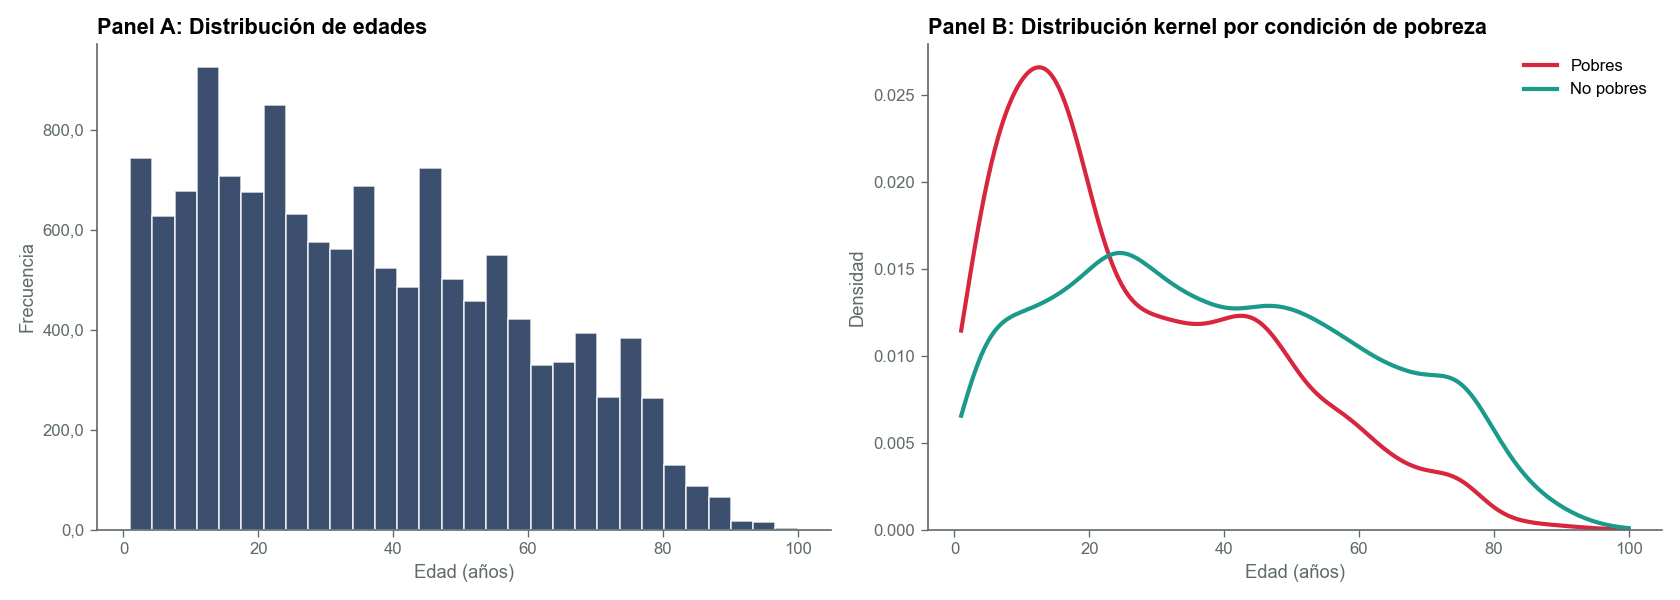
\includegraphics[width=1\textwidth]{../graficos/distribucion_edades_paneles.png}
    \caption{Distribución de edades: histograma general (Panel A) y distribuciones kernel por condición de pobreza (Panel B)}
    \label{fig:edades}
\end{figure}

\begin{figure}[htb!]
    \centering
    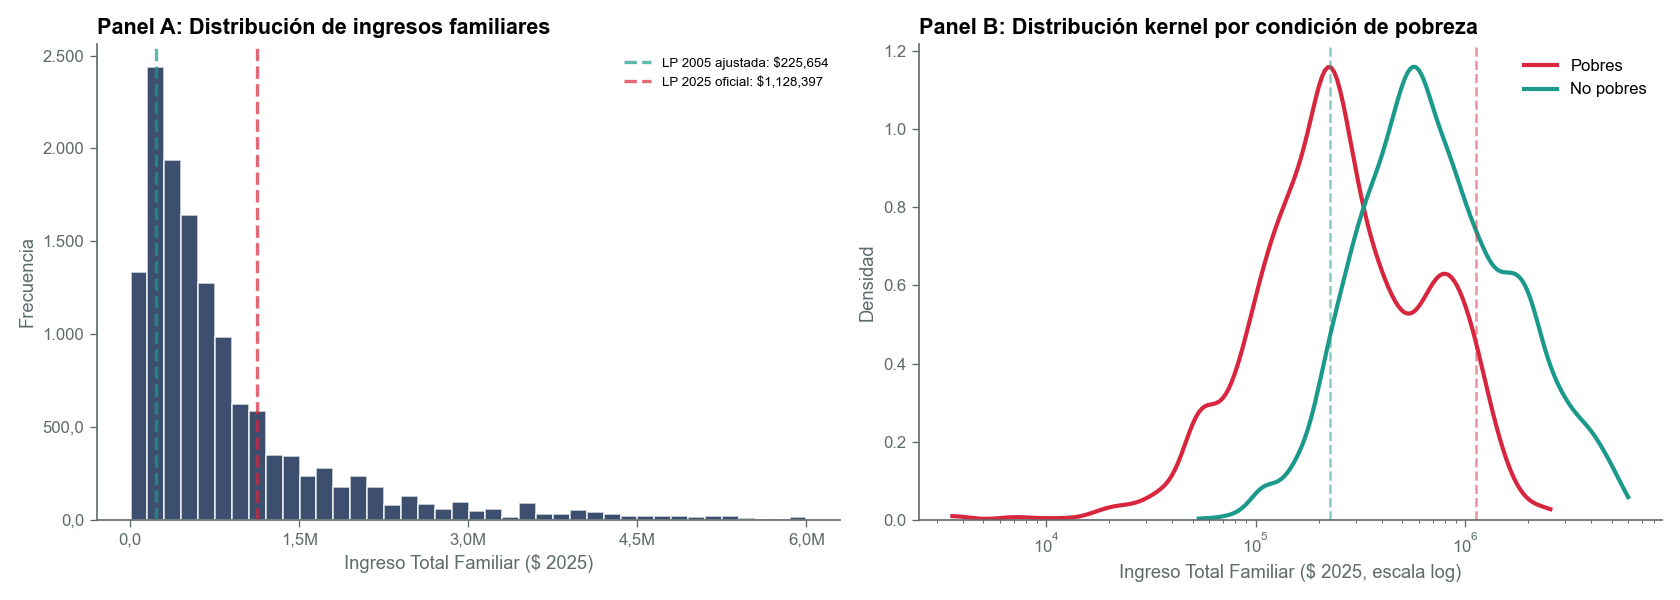
\includegraphics[width=1\textwidth]{../graficos/distribucion_ingresos_paneles.png}
    \caption{Distribución del ingreso total familiar: histograma general (Panel A) y distribuciones kernel por pobreza en escala logarítmica (Panel B)}
    \label{fig:ingresos}
\end{figure}

\begin{figure}[htb!]
    \centering
    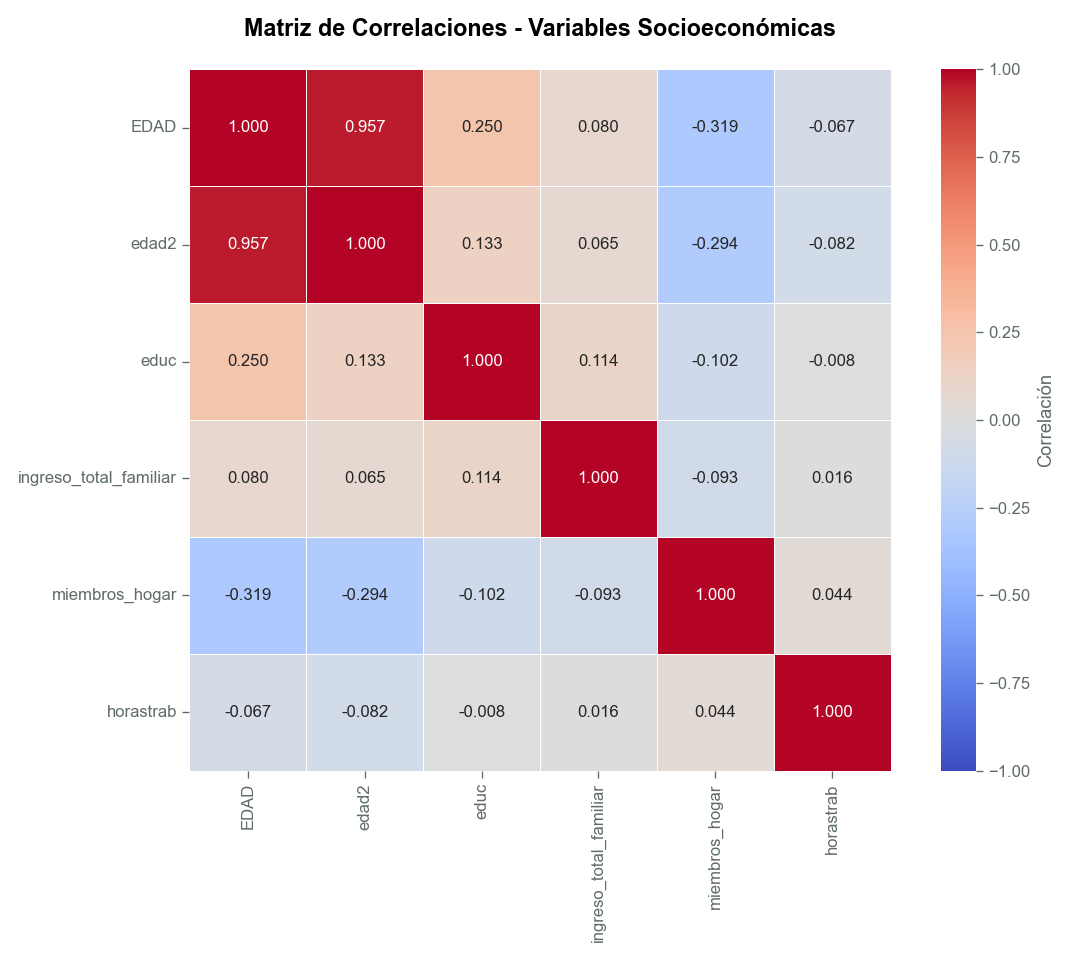
\includegraphics[width=0.85\textwidth]{../graficos/matriz_correlaciones.png}
    \caption{Matriz de correlaciones entre variables socioeconómicas seleccionadas}
    \label{fig:correlaciones}
\end{figure}

\begin{figure}[htb!]
    \centering
    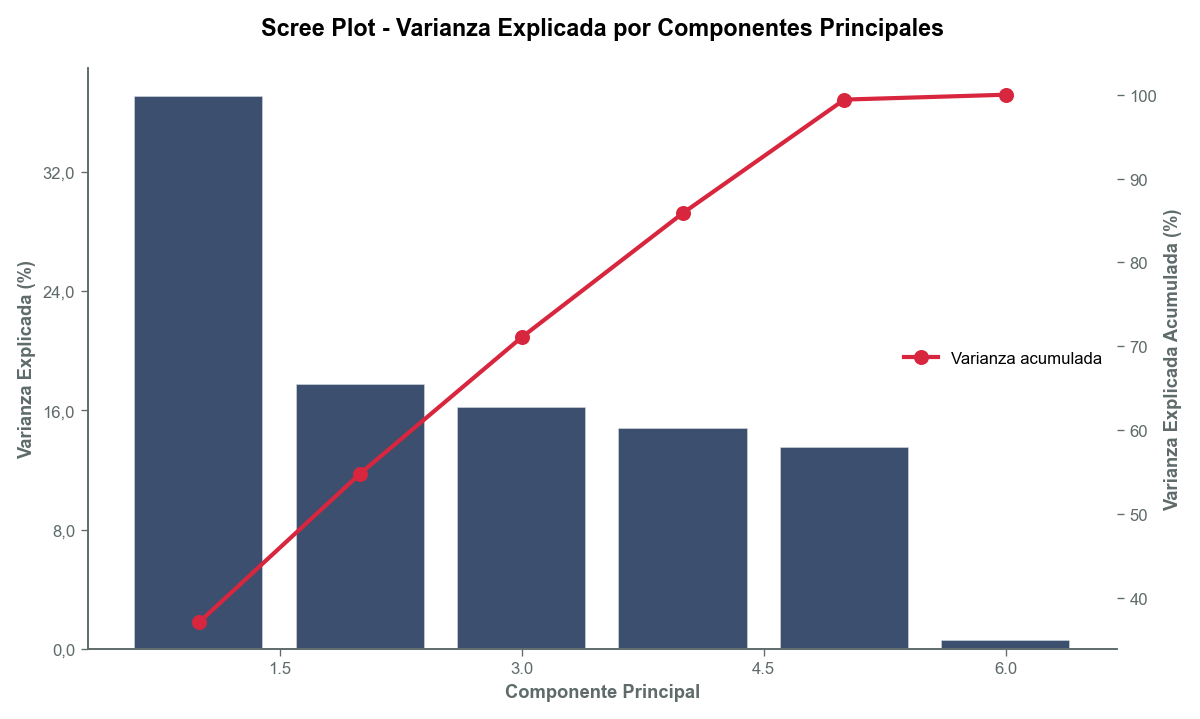
\includegraphics[width=0.9\textwidth]{../graficos/pca_scree_plot.png}
    \caption{Scree Plot: varianza explicada por cada componente principal (barras) y varianza acumulada (línea)}
    \label{fig:scree}
\end{figure}

\begin{figure}[htb!]
    \centering
    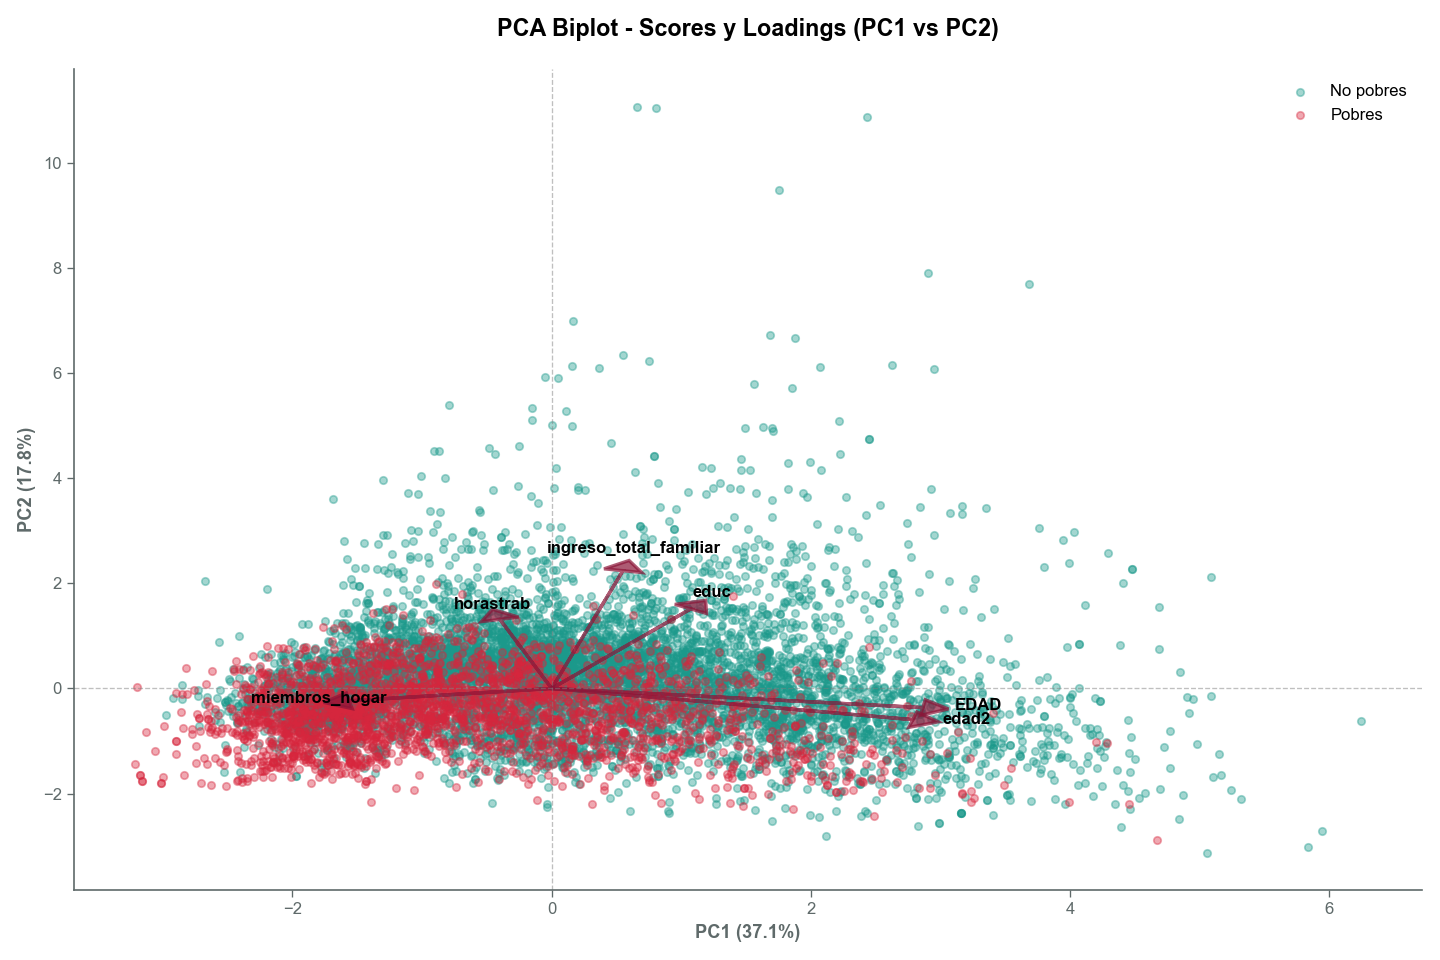
\includegraphics[width=1\textwidth]{../graficos/pca_biplot_scores.png}
    \caption{PCA Biplot: scores (puntos coloreados por pobreza) y loadings (vectores rojos) en espacio PC1-PC2}
    \label{fig:biplot}
\end{figure}

\begin{figure}[htb!]
    \centering
    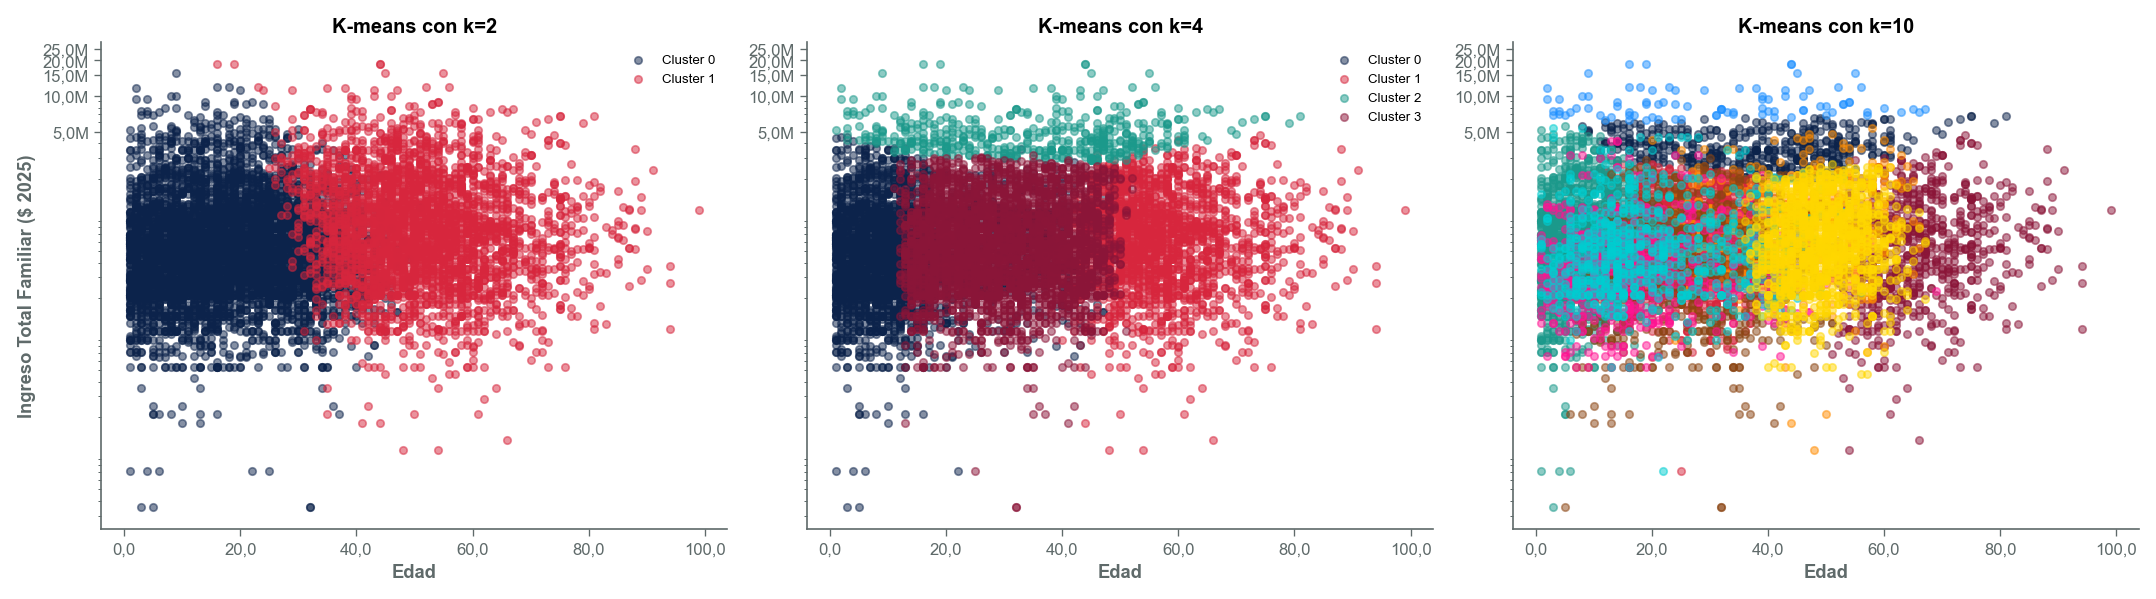
\includegraphics[width=1\textwidth]{../graficos/kmeans_clusters_edad_ingreso.png}
    \caption{Visualización de clusters K-means en espacio edad-ingreso para $k=2$, $k=4$ y $k=10$}
    \label{fig:clustersedadingreso}
\end{figure}

\begin{figure}[htb!]
    \centering
    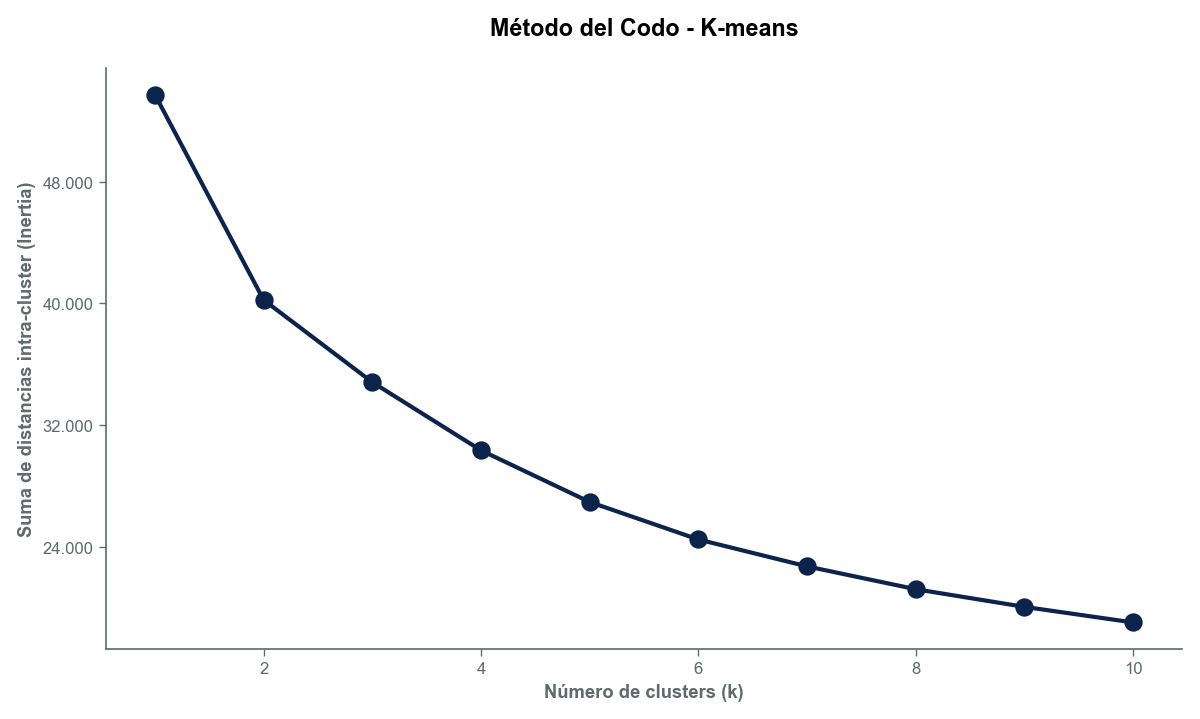
\includegraphics[width=0.9\textwidth]{../graficos/kmeans_elbow_method.png}
    \caption{Método del codo para determinar número óptimo de clusters en K-means}
    \label{fig:elbow}
\end{figure}

\begin{figure}[htb!]
    \centering
    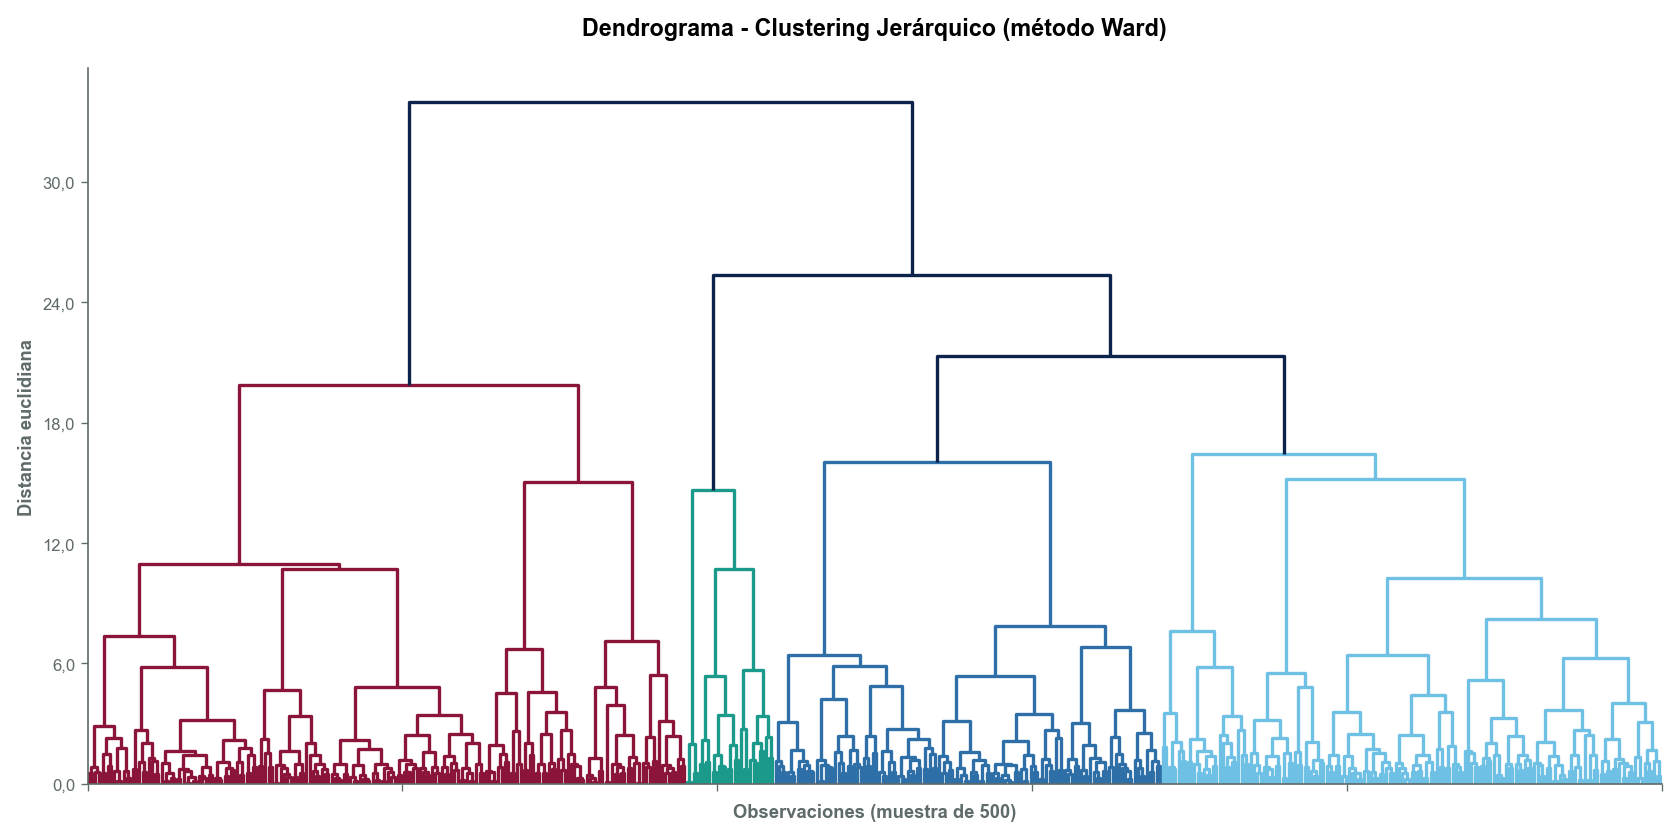
\includegraphics[width=1\textwidth]{../graficos/hierarchical_dendrogram.png}
    \caption{Dendrograma del clustering jerárquico con método Ward (muestra de 500 observaciones)}
    \label{fig:dendrograma}
\end{figure}

\begin{figure}[htb!]
    \centering
    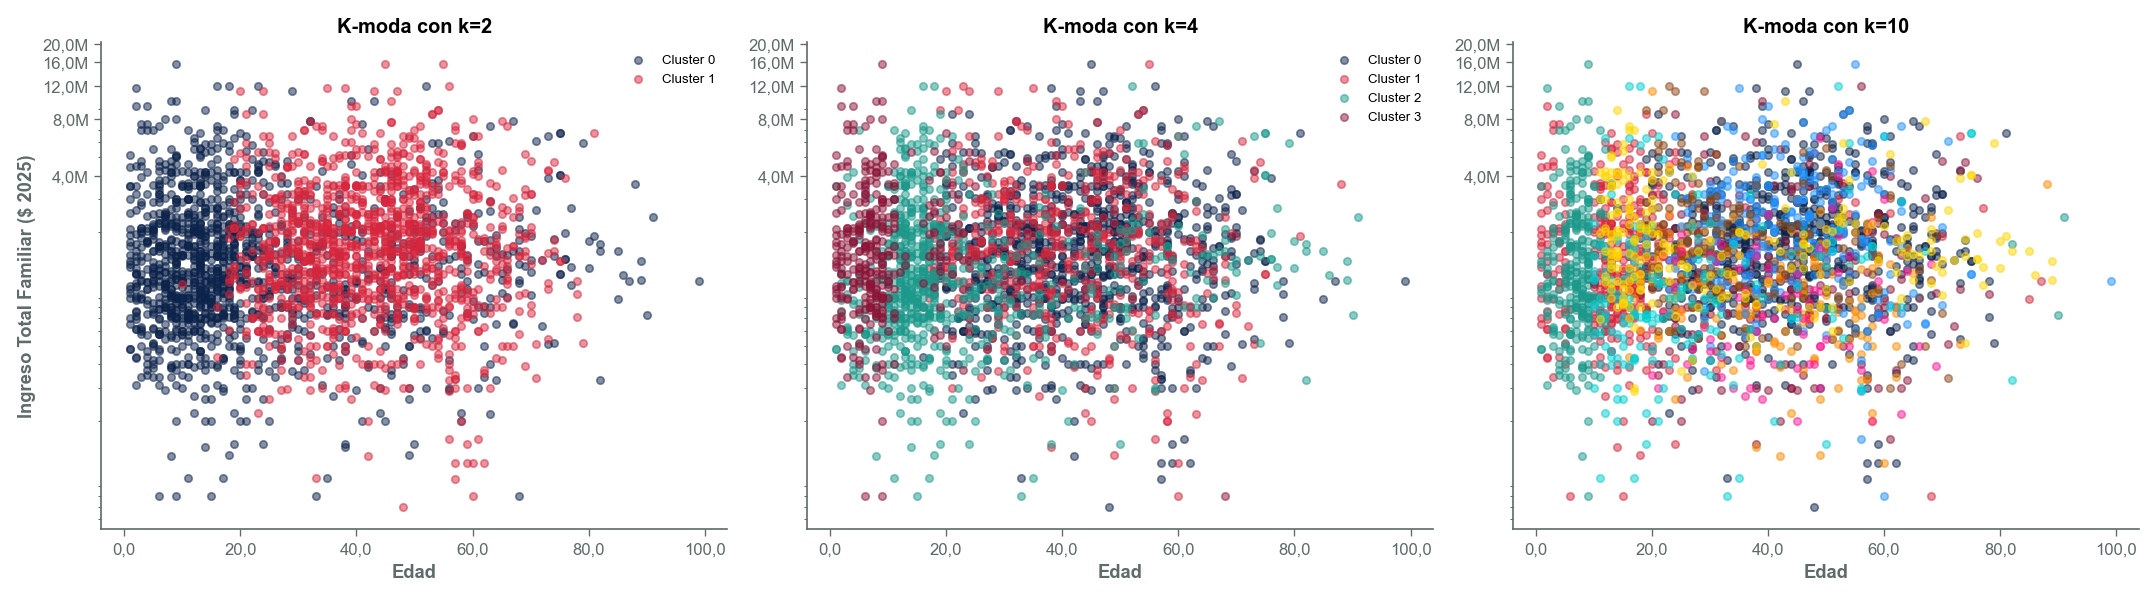
\includegraphics[width=1\textwidth]{../graficos/kmoda_clusters_edad_ingreso.png}
    \caption{Visualización de clusters K-moda (variables categóricas) proyectados en espacio edad-ingreso para $k=2$, $k=4$ y $k=10$}
    \label{fig:kmodaclusters}
\end{figure}

\end{document}
